\documentclass[11pt,a4paper]{article}

% ---------------------------------------------------------------------
% Packages
% ---------------------------------------------------------------------
\usepackage[T1]{fontenc}
\usepackage[utf8]{inputenc}
\usepackage{lmodern}
\usepackage[a4paper,margin=2.3cm]{geometry}
\usepackage{graphicx}
\usepackage{booktabs}
\usepackage{tabularx}
\usepackage{longtable}
\usepackage{array}
\usepackage{float}
\usepackage{caption}
\usepackage{enumitem}
\usepackage{xcolor}
\usepackage{fancyhdr}
\usepackage{amsmath}
\usepackage{listings}
\usepackage[hidelinks]{hyperref}

\setlength{\parskip}{0.45em}
\setlength{\parindent}{0pt}
\setlist{itemsep=0.15em,topsep=0.3em}
\captionsetup{font=small,labelfont=bf}
\newcolumntype{Y}{>{\raggedright\arraybackslash}X}
\renewcommand{\arraystretch}{1.15}

\lstset{basicstyle=\ttfamily\small,columns=fixed,basewidth=0.5em,frame=single,
        framerule=0.3pt,rulecolor=\color{gray},breaklines=true,
        xleftmargin=0.5em,xrightmargin=0.5em}


\pagestyle{fancy}
\fancyhf{}
\fancyhead[L]{\small DBMS Assignment 1: toyDB}
\fancyhead[R]{\small B24CS1056, B24CS1064}
\fancyfoot[C]{\small\thepage}
\renewcommand{\headrulewidth}{0.4pt}

% ---------------------------------------------------------------------
\begin{document}

% ---------------------------------------------------------------------
% Title page
% ---------------------------------------------------------------------
\begin{titlepage}
\centering
\vspace*{2.5cm}
{\Large Indian Institute of Technology Jodhpur\par}
\vspace{0.4cm}
{\large Database Management Systems\par}
\vspace{2cm}
{\huge\bfseries Assignment 1\par}
\vspace{0.4cm}
{\LARGE Buffer Management, Slotted Pages and\\[0.2em] B+ Tree Index Construction on toyDB\par}
\vspace{2.2cm}
\begin{tabular}{ll}
\toprule
\textbf{Name} & \textbf{Roll number} \\
\midrule
Pranav H Nair & B24CS1056 \\
Ridham Shah & B24CS1064 \\
\bottomrule
\end{tabular}\par
\vspace{1.6cm}
{\large Instructor: Nitin Awathare\par}
\vspace{0.3cm}
{\large Submitted: November 2026\par}
\vfill
{\small Submission file: \texttt{B24CS1056-B24CS1064.tar.gz}\par}
\end{titlepage}

\begin{abstract}
\noindent This report extends the Paged File (PF) and Access Method (AM) layers of toyDB in three ways. The buffer manager gains a configurable pool, LRU and MRU replacement chosen per file, an explicit dirty flag and exact I/O statistics. On a hot/cold workload LRU reaches a hit ratio of 0.307 against 0.124 for MRU, while on a looping sequential scan LRU has no hits at all and MRU reaches exactly the predicted 0.090 and 0.810. A heap file of slotted pages stores the 17{,}813 student records without loss at 95.0\% space utilization, against 86.8\% for the smallest lossless static layout and 36.1\% for a static limit of 256 bytes. A bulk loader for the B+ tree builds the roll-number index in 72 pages with 98.8\% full leaves, 35\% fewer pages than insertion, using 2 page reads and 73 page writes against 35{,}478 and 18{,}030, and the resulting index needs 41\% fewer physical reads per point query. Every result is regenerated by one command, every program is checked by tests with hand-computed expected values, and the quantities that follow from first principles match their predictions (Section~\ref{sec:validation}).
\end{abstract}
\newpage
{\setlength{\parskip}{0pt}\tableofcontents}
\newpage

% ---------------------------------------------------------------------
\section{Introduction}
% ---------------------------------------------------------------------

toyDB is a teaching database that provides the two lowest layers of a DBMS: the Paged File (PF) layer, which manages fixed-size pages of a file through a buffer pool, and the Access Method (AM) layer, which builds B+ tree indexes on top of the PF layer. This assignment extends both layers in three directions.

\begin{enumerate}
\item \textbf{Buffer management (Part 1).} A buffer pool whose size is a configuration parameter, LRU and MRU replacement selectable per file when it is opened, a dirty flag with an explicit call to mark a page modified, and statistics on logical and physical I/O. The statistics are measured for different mixtures of read and write queries and plotted.
\item \textbf{Slotted pages (Part 2).} A heap file of variable-length records in slotted pages, with insertion, deletion and sequential scan, used to store the student table. Its space utilization is compared with a static fixed-length layout for several maximum record lengths.
\item \textbf{Index construction (Part 3).} A B+ tree on the roll-number field of the student file, built from an existing file in one operation, incrementally through inserts, and by bulk loading from sorted input, compared on query completion time and pages accessed.
\end{enumerate}

Two principles shaped the implementation. First, the submission rules allow only the configuration file to change after submission, so every tunable of every experiment is a key in one file, \texttt{toydb.conf}, and no test depends on its values. Second, every result in this report is produced by a program in the repository and checked by a test with hand-computed expected values, so each number can be regenerated with one command (Appendix~\ref{app:build}).

Every modification of the provided PF and AM source is marked in the code with a comment \texttt{CHANGED [ID]} and listed with its reason and its consequence if omitted in Section~\ref{sec:changes}. Every other design decision is recorded with its reason and the consequence of not taking it in Appendix~\ref{app:decisions} (identifiers D1 to D37, cited in the text) and in \texttt{docs/DECISIONS.md} in the repository.

% ---------------------------------------------------------------------
\section{Build, configuration and testing infrastructure}
\label{sec:infra}
% ---------------------------------------------------------------------

\subsection{Building the provided code}

The provided sources are pre-ANSI C: implicit \texttt{int}, K\&R function definitions and calls to functions declared with an empty parameter list. Current compilers reject them in their default mode; under the default C23 mode of gcc 15.2, \texttt{pflayer/buf.c} fails with 32 errors, \texttt{pf.c} with 47 and \texttt{hash.c} with 19. A single top-level \texttt{Makefile} therefore compiles the provided sources with \texttt{-std=gnu89} and all new code with \texttt{-std=gnu89 -Wall -Wextra}, and the new code builds without a single warning (change B1).

The AM layer carried its own stale copy of \texttt{pf.h} with a page size of 1020 bytes, while the PF layer uses 4096. With the stale copy, B+ tree nodes used only a quarter of every page, which would have made every Part 3 page count roughly four times too large. The copy was removed so both layers share one header (change B2).

\subsection{Configuration}

All parameters are read from \texttt{toydb.conf}, a \texttt{key = value} file parsed by \texttt{common/config.c}. The file is located through a \texttt{conf=} argument, then the \texttt{TOYDB\_CONF} environment variable, then the current directory, and any key can be overridden on a program's command line as \texttt{key=value}. The keys cover the buffer pool size and default policy, the data file, the benchmark sizes, the static record lengths, seeds and repeat counts, and the bulk-load fill factor (Appendix~\ref{app:config}).

Because an evaluator may edit the configuration and then run the tests, \texttt{make test} must pass for any valid configuration. The configuration test therefore checks only that every key is present and parses; a stricter mode (\texttt{make test CONF\_MODE=exact}), used during development, also compares each key with its documented default. Benchmark self-tests use fixed fixtures rather than configuration values (D3, D4).

\subsection{Testing}

\texttt{make test} runs every test program in a scratch directory with a time limit and accepts a program only if its last output line is its expected completion line. Several provided test programs have no return statement, so exit codes alone would be meaningless (D5). Tests that need the student data resolve the configured path against the repository root and report a visible SKIPPED note if the file is absent (D6). Expected values in every test are computed by hand and written into the test, never copied from the program's own output (D7). Table~\ref{tab:tests} lists the test programs.

\begin{table}[H]
\centering
\small
\caption{Test programs run by \texttt{make test} (and \texttt{make stress}).}
\label{tab:tests}
\begin{tabularx}{\textwidth}{lY}
\toprule
Program & What it checks \\
\midrule
\texttt{amlayer/test1..3}, \texttt{amtest}, \texttt{pflayer/testpf} & The provided regression tests, unchanged. \\
\texttt{test\_config} & Parser, lookup order, overrides; every key of \texttt{toydb.conf} parses; malformed values are rejected. \\
\texttt{test\_pool} & Runtime pool sizing, minimum size, resizing only while the pool is empty. \\
\texttt{test\_policy} & Exact LRU and MRU victim order, per-file policies sharing one pool. \\
\texttt{test\_dirty} & \texttt{PF\_MarkDirty}, write-back on eviction and close, loss of unmarked changes. \\
\texttt{test\_stats} & Every counter against hand-computed values, attribution to the right file. \\
\texttt{test\_workload} & An LRU versus MRU workload with known outcome. \\
\texttt{stress\_pool} & Randomized test of every PF call against an independent model of the buffer rules (20 seeds; \texttt{make stress}). \\
\texttt{bench\_buffer check} & 162 assertions on small fixtures, including hand-traced LRU and MRU counts. \\
\texttt{test\_hfpage}, \texttt{test\_hf} & Slotted page operations; heap file insert, get, delete, scan, reopen. \\
\texttt{test\_hf\_load} & Loads \texttt{student.txt}; every record reads back byte for byte; statistics consistent. \\
\texttt{test\_hfstatic} & Static layout: stored lengths, truncation flag, slot reuse, exact statistics. \\
\texttt{bench\_space check} & Space statistics of both layouts on hand-computed fixtures. \\
\texttt{test\_leftpage} & B+ tree scans on insert-built and bulk-style trees (changes A1, A3). \\
\texttt{test\_amscan} & Every scan operator on every key, gap value and bound, seven trees (changes A4 to A7). \\
\texttt{test\_ambulk}, \texttt{test\_bulk} & Bulk loader: hand-computed shapes, fill factors, duplicates, record-id limit, scans, inserts after loading, no unreachable page. \\
\texttt{test\_bulk\_data} & Bulk-loads the roll-number index from \texttt{student.txt}; every key found with its record ids. \\
\texttt{bench\_index check} & Index benchmark on 604 synthetic records with hand-computed shape and result counts. \\
\bottomrule
\end{tabularx}
\end{table}

Before submission the complete repository was checked once more, in a fresh clone, by an audit independent of the tests above. The code builds without warnings at \texttt{-O0}, \texttt{-O1} and \texttt{-O2}, and all 23 programs of \texttt{make test} pass both under AddressSanitizer and UndefinedBehaviorSanitizer, with no leaks, and under valgrind, with no invalid reads or writes. The only valgrind reports are uninitialised padding bytes of stack structures that the provided \texttt{AM\_CreateIndex} and \texttt{AM\_SplitLeaf} copy into index pages; these bytes are never read back, so the provided code was left unchanged. Every valid configuration tried (pool sizes from the minimum of 8 to 100{,}000 frames, both policies, fill factors from 0.01 to 1.0, absolute and relative data paths, a path containing a space) passes \texttt{make test}, and every invalid value stops the program with status 1 and names the key. Seventeen edge-case data files (empty, header only, LF line endings, no final newline, wrong field counts, an over-long record, sorted and reverse-sorted keys, one record, exactly one full leaf, and one key repeated up to 700 times) run through the four data programs without a crash, a hang or a wrong count, the last case with a clear error once a key exceeds 677 record ids. Rerunning all three benchmarks reproduces every page and I/O count of the committed results, and the packaged archive builds and passes its tests with and without the data file.

% ---------------------------------------------------------------------
\subsection{Experimental setup}
\label{sec:setup}

All measurements in this report were taken on the machine in Table~\ref{tab:setup}. All programs are single-threaded. Physical reads and writes are page transfers between the buffer pool and the file through the operating system's read and write calls, so they count the I/O requested by the DBMS. Whether the operating system served a read from its own file cache or from the SSD is not visible to the program, which is why page counts rather than times are the primary metric (D37).

\begin{table}[H]
\centering
\small
\caption{Experimental platform.}
\label{tab:setup}
\begin{tabularx}{\textwidth}{lY}
\toprule
Component & Value \\
\midrule
Processor & Intel Core i5-1235U, 10 cores (2 performance, 8 efficiency), 12 threads \\
Memory & 6.9 GiB available to the operating system \\
Storage & Western Digital PC SN740, 512 GB NVMe SSD \\
Operating system & Ubuntu Linux, kernel 6.17 \\
Compiler & gcc 15.2.0; provided code \texttt{-std=gnu89 -O2 -g -w}, new code \texttt{-std=gnu89 -O2 -g -Wall -Wextra} \\
Plotting & Python 3 with matplotlib 3.10.1 \\
Page size & 4096 bytes (\texttt{PF\_PAGE\_SIZE}) \\
\bottomrule
\end{tabularx}
\end{table}

% ---------------------------------------------------------------------
\section{Part 1: Buffer manager}
\label{sec:part1}
% ---------------------------------------------------------------------

\subsection{Design}

\paragraph{Pool size.} The compile-time pool of 20 frames was replaced by a pool allocated at run time. \texttt{PF\_Init} sizes it from \texttt{buffer\_pool\_size}, and \texttt{PF\_InitBuffer(n)} resizes it while no page is resident; the minimum is 8 frames (change P1). The page hash table was enlarged from 20 to 1031 buckets so that lookups stay short for pools of hundreds of frames (P2).

\paragraph{Replacement policy per file.} Each open-file entry records a policy. \texttt{PF\_OpenFileEx(name, PF\_LRU)} or \texttt{PF\_OpenFileEx(name, PF\_MRU)} selects it, and \texttt{PF\_OpenFile(name)} is kept as a wrapper that uses the configured default, so existing callers are unchanged (P3, P4). The pool remains shared by all files, so the policy that chooses a victim is the policy of the file whose page is being brought in, and the victim may belong to any open file (D8).

\paragraph{Recency.} The buffer keeps the provided doubly linked list with the most recently used page at the head. A page moves to the head when it is loaded and when it is unfixed; a hit does not move it. LRU evicts the first unfixed page from the tail and MRU the first unfixed page from the head (D9). This definition keeps the change to the provided code small and gives an exact order that the tests can check. MRU suits sequential access: the page a scan has just released sits at the head, so MRU evicts it and keeps the rest of the pool, which is exactly the case where LRU evicts every page just before it is needed again.

\paragraph{Dirty flag.} Each frame has a dirty flag. It is set by an unfix with \texttt{dirty = TRUE}, by the new call \texttt{PF\_MarkDirty(fd, page)}, or by page allocation, and an unfix with \texttt{dirty = FALSE} never clears it, so an earlier modification cannot be lost (P5, D10). \texttt{PF\_MarkDirty} does not change recency. Dirty pages are written back on eviction, on close, and by the new \texttt{PF\_FlushAll}.

\paragraph{Statistics.} The layer keeps eight counters per open file and a global total, read with \texttt{PF\_GetStats} and cleared with \texttt{PF\_ResetStats} (P6). Table~\ref{tab:counters} defines them. Reads, hits, misses and logical writes are charged to the file of the requested page; evictions and physical writes to the file of the victim. A logical write is counted at most once per fix of a page, so marking a page dirty twice before unfixing it is one write (D11). With these definitions \(\textit{hits} + \textit{misses} = \textit{logical reads}\) holds exactly, and every test and every benchmark run checks it.

\begin{table}[H]
\centering
\small
\caption{Buffer statistics kept per file and globally.}
\label{tab:counters}
\begin{tabularx}{\textwidth}{lY}
\toprule
Counter & Meaning \\
\midrule
\texttt{logical\_reads} & Requests to fix an existing page, hit or miss. \\
\texttt{hits} & Logical reads whose page was already in the pool. \\
\texttt{misses} & Logical reads whose page had to be read from the file. \\
\texttt{physical\_reads} & Pages read from the file into a frame. \\
\texttt{logical\_writes} & Requests to mark a page dirty, at most one per fix of the page. \\
\texttt{physical\_writes} & Pages written to the file on eviction, on close or by \texttt{PF\_FlushAll}. \\
\texttt{evictions} & Frames taken from a resident page to make room. \\
\texttt{dirty\_evictions} & Evictions whose victim was dirty and was written back. \\
\bottomrule
\end{tabularx}
\end{table}

\subsection{Verification}

Five test programs check the buffer manager against hand-computed scenarios: exact victim order for both policies, write-back and the loss of an unmarked change, and every counter including its attribution between files. In addition, \texttt{stress\_pool} drives random sequences of every PF call (fix, unfix clean and dirty, mark dirty, page modification, flush, close and reopen, and deliberate misuse) against an independent model written from the documented rules, with two files of different policies sharing pools of random size. It compares every return code, the set of resident pages, all counters and finally the disk contents. All 20 seeds pass at 200{,}000 and at 2{,}000{,}000 operations, and seeds 1 and 2 at 2{,}000{,}000 operations are also clean under AddressSanitizer and UndefinedBehaviorSanitizer. With one model rule deliberately broken (the LRU victim taken from the wrong end of the list), the test fails within the first few thousand operations, which shows that it can detect a wrong replacement order (D7).

The stress test also exposed one undocumented behaviour of the provided code: closing a file that still has a fixed page returns \texttt{PFE\_PAGEFIXED} after already writing back and releasing that file's unfixed pages that precede the fixed one in the list. No requirement depends on it, so it was documented and left unchanged (D12).

\subsection{Experiment}

The benchmark (\texttt{make bench}) works on a file of 1000 pages. An operation fixes one page and unfixes it; a read unfixes it clean, and a write modifies one byte and marks the page dirty (alternately through \texttt{PF\_UnfixPage(\ldots, TRUE)} and through \texttt{PF\_MarkDirty}, so both paths are measured). Each run performs 10{,}000 operations on a cold pool. The runs cover:

\begin{itemize}
\item pool sizes of 20, 50, 100, 900 (close to the file size) and 1200 frames (larger than the file);
\item three access patterns: \emph{uniform} (random page, a control on which LRU and MRU should perform alike), \emph{hot/cold} (80\% of accesses to 20\% of the pages, which favours LRU) and \emph{sequential} (a looping scan over all pages, the worst case of LRU, which favours MRU);
\item read percentages of 100, 90, 75, 50, 25, 10 and 0;
\item both policies and five repeats with different seeds, 1050 runs in total (D13).
\end{itemize}

For a fair comparison, LRU and MRU and every pool size see exactly the same sequence of pages. The page sequence is also independent of the read percentage: one random generator chooses pages and a second one decides between read and write. Replacement ignores the dirty flag, so with the same page sequence the hits, misses, physical reads and evictions are identical at every read mix, and the graphs isolate the effect of the write mix. This holds in all 150 groups of runs in the results (D14). Physical writes are reported twice, before and after a final \texttt{PF\_FlushAll}; without the flush, a pool larger than the file would show no physical writes even for an all-write workload, as if writes cost nothing (D15).

\subsection{Results}

\begin{figure}[H]
\centering
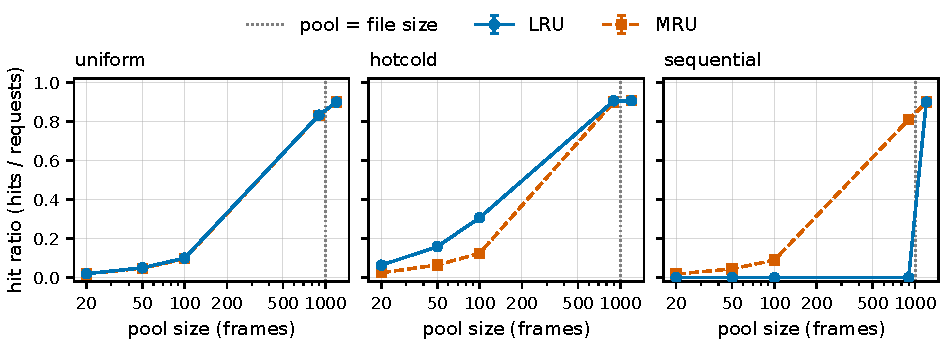
\includegraphics[width=\textwidth]{figures/buffer_hit_ratio.pdf}
\caption{Hit ratio against pool size (log scale) for all-read workloads, means of five repeats with min/max bars. The dotted line marks a pool equal to the file size (1000 pages).}
\label{fig:hitratio}
\end{figure}

\begin{figure}[H]
\centering
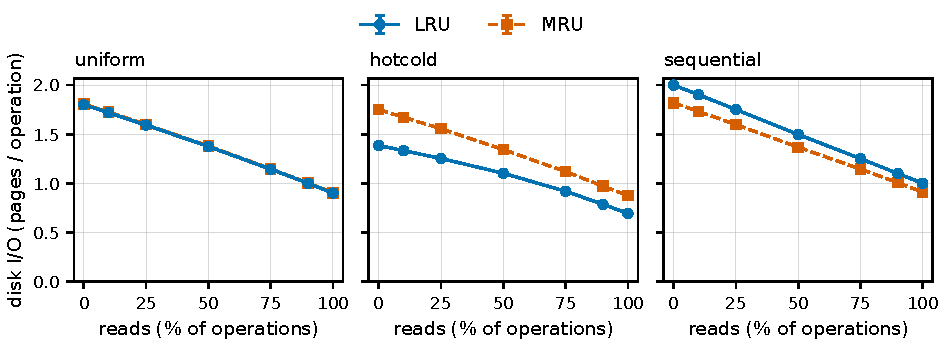
\includegraphics[width=\textwidth]{figures/buffer_io_vs_mix.pdf}
\caption{Disk I/O per operation, (physical reads + physical writes after the final flush) / operations, against the percentage of read queries, at a pool of 100 frames.}
\label{fig:iomix}
\end{figure}

\begin{figure}[H]
\centering
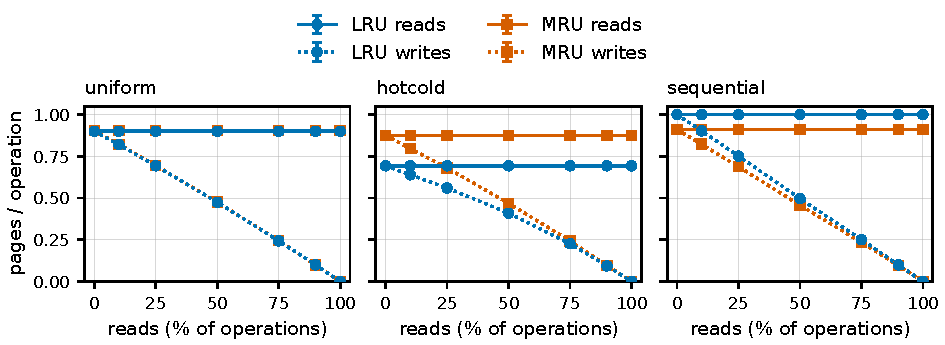
\includegraphics[width=\textwidth]{figures/buffer_io_breakdown.pdf}
\caption{The disk I/O of Figure~\ref{fig:iomix} split into physical reads (solid) and physical writes (dotted) per operation, at a pool of 100 frames.}
\label{fig:iobreak}
\end{figure}

\begin{table}[H]
\centering
\small
\caption{Pool of 100 frames, 50\% reads, 10{,}000 operations; means over five repeats.}
\label{tab:buffersummary}
\begin{tabular}{llrrrrr}
\toprule
Pattern & Policy & Hit ratio & Phys.\ reads & Phys.\ writes & Evictions & Dirty evict. \\
\midrule
uniform & LRU & 0.100 & 9001.0 & 4746.6 & 8901.0 & 4689.2 \\
 & MRU & 0.097 & 9032.6 & 4759.6 & 8932.6 & 4708.6 \\
\midrule
hot/cold & LRU & 0.307 & 6930.4 & 4091.4 & 6830.4 & 4030.4 \\
 & MRU & 0.124 & 8756.6 & 4683.2 & 8656.6 & 4633.0 \\
\midrule
sequential & LRU & 0.000 & 10000.0 & 4974.8 & 9900.0 & 4926.2 \\
 & MRU & 0.090 & 9100.0 & 4571.6 & 9000.0 & 4473.0 \\
\bottomrule
\end{tabular}
\end{table}

\subsection{Discussion}

\paragraph{Uniform access.} With uniformly random pages the expected hit ratio of any policy is the fraction of the file the pool can hold. At 100 frames LRU reaches 0.100 and MRU 0.097, against an expected 100/1000; the two curves of Figure~\ref{fig:hitratio} coincide at every pool size. This control shows that the measurement favours neither policy.

\paragraph{Hot/cold access.} When 80\% of the accesses go to 200 hot pages, LRU keeps the hot pages because they are reused before they reach the tail of the list, while MRU evicts the page it has just used, which is most likely hot. At 100 frames LRU reaches a hit ratio of 0.307 against 0.124 for MRU, and at 50 frames 0.159 against 0.065. At a pool of 100 frames LRU therefore needs 21\% fewer physical reads than MRU (6930 against 8757 for 10{,}000 operations at 50\% reads).

\paragraph{Sequential access.} A looping scan over 1000 pages is the classic worst case of LRU: each page is evicted just before the scan returns to it, so LRU has no hits at all for any pool smaller than the file, including 900 frames. MRU evicts the page just released and keeps the rest of the pool, so after the first pass it hits on as many pages per pass as the pool holds; with 10 passes this gives exactly \(9 \times 100 / 10\,000 = 0.090\) at 100 frames and \(9 \times 900 / 10\,000 = 0.810\) at 900 frames, the measured values. Once the pool holds the whole file (1200 frames), the two policies coincide on every pattern; for uniform and sequential access the hit ratio is 0.900, the limit set by the 1000 compulsory misses (hot/cold reaches 0.907 because some cold pages are never touched).

\paragraph{Read and write mixtures.} Figure~\ref{fig:iobreak} shows the central result of the mixture experiment: physical reads per operation are flat across the read percentage, and only physical writes change, falling linearly to zero as the share of reads grows. The replacement policy decides how many pages must be read; the mixture decides how many evicted pages are dirty and must be written back. Total disk I/O (Figure~\ref{fig:iomix}) therefore rises linearly with the share of writes, from 0.90 pages per operation for an all-read uniform workload to 1.80 for an all-write one. The policy that wins on reads also wins on writes: for hot/cold at 0\% reads LRU needs 1.39 pages per operation and MRU 1.75, and for the sequential scan LRU reaches 2.00, one read and one write-back for every operation. Logical I/O is one request per operation in every run.

\paragraph{Choice of policy.} No single policy is best. LRU suits workloads with a reused working set, MRU suits repeated sequential scans of a file larger than the pool, and the per-file choice at open time allows each file to use the policy that matches its access pattern while sharing one pool.

% ---------------------------------------------------------------------
\section{Part 2: Slotted pages and static record management}
\label{sec:part2}
% ---------------------------------------------------------------------

\subsection{Data}

\texttt{student.txt} contains a title line, 17{,}813 records of 16 semicolon-separated fields and a final empty line, with Windows (CRLF) line endings. A record is the content of one line without its line terminator; the loader strips the carriage return as well as the newline and skips lines that do not have 16 fields (D19). The records are 1{,}759{,}011 bytes in total, with a mean length of 98.75 bytes and a maximum of 108 bytes. The narrow range of lengths matters for the comparison below.

\subsection{Slotted page layout}

The heap file reserves page 0 for metadata (number of data pages and of records). Each data page has a 4-byte header (slot count and start of the record area), a slot directory that grows from the front with one 4-byte entry (offset and length) per slot, and record bytes that grow backwards from the end of the page. A deleted record leaves an empty slot so that the record ids of the other records on the page do not change; the records of a page may be compacted to gather free space. A record id is \(\textit{page} \times 4096 + \textit{slot}\), a single non-negative integer that the B+ tree can store unchanged (D17). An insertion takes the first page with enough contiguous free space, so space freed by deletions is reused. The file supports insertion, retrieval and deletion by record id and a sequential scan.

\subsection{Static layout}

The static baseline gives every record a slot of fixed size. To store variable-length records in fixed slots, each slot holds a 2-byte length word followed by \(L\) bytes of data: the low 15 bits give the stored length, the top bit marks a record that was truncated to \(L\) bytes, and the value \texttt{0xFFFF} marks an empty slot. With a 4-byte page header,
\[
\textit{slots per page} = \left\lfloor \frac{4096 - 4}{L + 2} \right\rfloor .
\]
Records longer than \(L\) are truncated and counted. Without the stored length, a short record would read back padded to \(L\) bytes and its true size would be lost (D21).

\subsection{Metric}

Both layouts use the same definitions, with the metadata page excluded: \emph{useful bytes} are the bytes of record content actually stored, and
\[
\textit{utilization} = \frac{\textit{useful bytes}}{\textit{data pages} \times 4096}.
\]
Using one definition is essential; counting slot capacity instead of stored data would credit the static layout with the padding it wastes (D18).

\subsection{Results}

Table~\ref{tab:space} gives the result of loading all 17{,}813 records (\texttt{make bench-space}). The benchmark also deletes 30\% of the records, chosen at random, and inserts them again; for both layouts this gives exactly the same pages, stored bytes and truncation counts as the first load, so both reuse freed space completely (D23).

\begin{table}[H]
\centering
\small
\caption{Space utilization of the slotted and static layouts for 17{,}813 student records. Records per page is the average, \(\lfloor \textit{records} / \textit{pages} \rfloor\).}
\label{tab:space}
\begin{tabular}{lrrrrrrr}
\toprule
Layout & \(L\) & Slots/page & Truncated & Data pages & Useful bytes & Records/page & Utilization \\
\midrule
slotted & -- & -- & 0 & 452 & 1\,759\,011 & 39 & 0.950 \\
\midrule
static & 100 & 40 & 5\,749 & 446 & 1\,748\,550 & 39 & 0.957 \\
static & 104 & 38 & 159 & 469 & 1\,758\,761 & 37 & 0.916 \\
static & 110 & 36 & 0 & 495 & 1\,759\,011 & 35 & 0.868 \\
static & 128 & 31 & 0 & 575 & 1\,759\,011 & 30 & 0.747 \\
static & 160 & 25 & 0 & 713 & 1\,759\,011 & 24 & 0.602 \\
static & 200 & 20 & 0 & 891 & 1\,759\,011 & 19 & 0.482 \\
static & 256 & 15 & 0 & 1\,188 & 1\,759\,011 & 14 & 0.361 \\
\bottomrule
\end{tabular}
\end{table}

\subsection{Discussion}

The slotted layout stores every record whole at 95.0\% utilization. Its overhead is the 4-byte slot entry per record and the 4-byte page header, about 162 bytes per page, plus the unused tail of each page.

A static layout can store every record whole only if \(L\) is at least the longest record, 108 bytes. The smallest such length in the experiment, 110, needs 495 pages against 452 for the slotted file, 9.5\% more, because every record occupies 112 bytes while the average record has 98.75. The waste grows linearly with \(L\): at \(L = 256\), a generous bound for a table whose longest record is 108 bytes, utilization falls to 36\% and the file needs 2.6 times as many pages. A static layout must choose \(L\) in advance from the longest record that may ever occur, and every shorter record pays for that choice.

The two shortest lengths show the other side of the trade-off. At \(L = 100\) the static file reaches 95.7\% utilization, slightly above the slotted file, only because 5{,}749 records (32\% of the table) lose their tail bytes; at \(L = 104\), 159 records are truncated. A higher utilization obtained by discarding data is not a valid gain. The slotted layout is therefore the only layout in the experiment that is both lossless and dense; a static layout matches it only when record lengths are nearly constant, and its cost grows with the spread between the average and the maximum length.

\subsection{Verification}

\texttt{test\_hf\_load} reads every loaded record back by record id and through a full scan and compares it byte for byte, and checks that the statistics agree with what was inserted. These checks are invariants rather than the numbers of this particular file, so the tests remain valid if the data file is changed (D20). The static layout was additionally tested with randomized sequences of 50{,}000 insertions, deletions, retrievals, scans and reopenings for slot lengths from 1 to 1024 bytes against an in-memory model, under sanitizers. An adversarial review of the first version found that the static statistics counted slot capacity instead of stored bytes, which reversed the comparison, and that the loaders kept the carriage return in every record; both were corrected before the results above were produced.

% ---------------------------------------------------------------------
\section{Part 3: B+ tree index construction}
\label{sec:part3}
% ---------------------------------------------------------------------

\subsection{Index key}

The index is built on the roll number, field 2 of the student file, as an 8-byte character key. An integer key would reject the alphanumeric roll numbers in the data (for example \texttt{96D07001}) and lose leading zeros (\texttt{01403310}) (D24). Three roll numbers occur twice; the AM layer stores a duplicate key as one entry with a list of record ids, so the index accepts them. The record id stored with each key is the record's heap-file id from Part 2.

\subsection{Corrections to the AM layer}

Six defects in the provided AM scan code had to be corrected before an index could be measured reliably. None of them causes a crash in ordinary use; each returns plausible but wrong results, and several leave pages fixed in the buffer pool.

\begin{itemize}
\item \textbf{Leftmost leaf (A1).} \texttt{GetLeftPageNum}, which full scans and the \(<\), \(\le\) and \(\ne\) scans use as their starting point, returned page 2 whenever the root was not a leaf. That holds only for trees built by insertion, where the first root split places the left half in page 2. In a tree whose leaves start at page 1, as in a bulk-loaded tree, a full scan returned 75 of 100 keys without any error. The function now descends the leftmost child pointers from the root.
\item \textbf{Not-equal skip (A3).} A \(\ne\) scan returned the key it should exclude, on insert-built trees as well, because skipping the key did not update the stored copy of the current key and a later consistency check undid the skip.
\item \textbf{Not-equal on an absent value (A4).} The scan cursor was never initialised, so the scan started from whatever an earlier scan had left in its slot: garbage results or a crash.
\item \textbf{Absent value after the last key of a leaf (A5).} When the search ended past the last key of a non-last leaf, the scan moved to the next leaf but released the wrong page, failing with a PF error and leaving two pages fixed. This is the case of a missing-key query that falls in the gap between two leaves, which the Part 3 workload asks for deliberately.
\item \textbf{\(\le\) on the largest key (A6)} undid its own end-of-scan state and read past the last leaf.
\item \textbf{\(<\) on the first key of a leaf (A7)} compared page numbers as if they were in leaf order; in insert-built trees they are not, so the scan stopped early and returned nothing.
\end{itemize}

A1 and A3 were found by \texttt{tests/test\_leftpage}, which builds trees with different page layouts. A4 to A7 were found by a randomized review of the bulk loader and confirmed on purely insert-built trees with the original AM code. \texttt{tests/test\_amscan} checks every operator on every key, every gap value and both bounds for seven trees: before the fixes all 4{,}807 not-equal probes on absent values, all 95 gap probes, all 7 \(\le\)-on-maximum probes and 5 of 19 \(<\)-on-first-key probes failed, while the 52{,}721 other probes passed before and after, showing that the fixes change only the broken paths.

\subsection{The bulk loader}

\texttt{AM\_BulkLoad} (\texttt{amlayer/ambulk.c}, change A2) receives (key, record id) pairs in sorted order through a callback, checks the order with the AM's own comparison, and builds the tree bottom-up with the AM's own page routines. Leaves are written left to right in pages \(1 \ldots k\) and chained; each internal level is built from the smallest key of each child; the root is written into page 0, where the AM layer expects it (D27). With fill factor \(f\) (\texttt{bulk\_fill\_factor}):
\[
\textit{leaf target} = \max\!\left(2, \lfloor f \cdot \textit{leaf capacity} \rfloor\right), \qquad
\textit{leaf capacity} = \left\lfloor \frac{4096 - 24}{L + 8} \right\rfloor = 254 \text{ for } L = 8,
\]
since a key with one record id costs \(L + 2\) bytes for the key entry and 6 bytes for the record-id node, and a leaf header is 24 bytes. Internal nodes take \(\max(3, \lfloor f \cdot 341 \rfloor)\) children. A key's record ids never span two leaves, so one key may have at most 677 record ids.

The first version of the loader passed its own tests but a review with a page dumper and a randomized model test found two errors that would have biased Part 3: the root was built in a spare page and copied into page 0, leaving an unreachable page in every index (73 pages instead of 72), and the leaf target was computed from the internal-node capacity (340) instead of the leaf capacity (254), so a fill factor of 0.75 built the same tree as 1.0. After the fix the student index has 72, 95 and 142 pages at fill factors 1.0, 0.75 and 0.5, every page reachable from the root, and the model test reports no mismatch over about 376{,}000 checks per seed.

\subsection{Build methods}

\begin{itemize}
\item \textbf{M1, existing file.} The heap file is already loaded (not measured). One scan of it inserts every (roll number, record id) with \texttt{AM\_InsertEntry}.
\item \textbf{M2, incremental.} Starting from an empty heap file and an empty index, each record is inserted into the heap file and its key into the index immediately.
\item \textbf{M3, bulk load.} One heap scan collects the pairs, they are sorted in the AM's key order, and \texttt{AM\_BulkLoad} builds the tree. The scan and sort are timed apart from the load; the load alone is the cost when the file is already sorted.
\end{itemize}

M2 runs first, and its heap file is the one indexed by M1 and M3, so all three indexes hold the same pairs.

\subsection{Measurement method}

\begin{itemize}
\item \textbf{Index and heap I/O are counted separately.} The PF counters charge every page access, including the write-back of an evicted dirty page, to the file that owns the page. This matters because the slotted heap insertion of Part 2 is first-fit and reads many heap pages; counted together, heap cost would dominate the comparison of the indexes. For every build the global counter delta must equal index plus heap I/O, and hits plus misses must equal logical reads; any difference stops the run (D32).
\item \textbf{Cold pool.} Every build and every query batch starts with all files closed and an empty pool of 50 frames (D34).
\item \textbf{Identical queries.} One query set per repeat is answered by all three indexes: 1000 point queries on existing keys, 100 queries on absent keys (half in the gap between two leaves, half inside a leaf), 200 range queries returning 100 record ids from an existing key, and one full scan (D33).
\item \textbf{Correctness.} Every query result is compared with a sorted in-memory copy of the pairs. All three indexes must pass, so they return identical answers.
\end{itemize}

Means over 5 repeats are reported; build I/O and tree shapes were identical in every repeat and only times varied. \texttt{bench\_index check}, run by \texttt{make test}, verifies the program on 604 synthetic records with a hand-computed shape and result counts.

\subsection{Results}

\begin{table}[H]
\centering
\small
\caption{Index construction and query cost on 17{,}813 student records, pool of 50 frames, fill factor 1.0; means over five repeats. Logical reads count page requests, physical reads and writes count page transfers between the pool and the file.}
\label{tab:index}
\begin{tabular}{lrrr}
\toprule
 & M1 existing & M2 incremental & M3 bulk \\
\midrule
Index pages & 110 & 110 & 72 \\
Leaves & 109 & 109 & 71 \\
Height & 2 & 2 & 2 \\
Leaf fill (\%) & 64.3 & 64.3 & 98.8 \\
\midrule
Build time (ms) & 8.4 & 2001.9 & 6.6 \\
\quad index part (ms) & 4.3 & 23.2 & 1.3 \\
\quad heap scan and sort (ms) & -- & -- & 5.3 \\
Build: index logical reads / writes & 35\,478 / 18\,030 & 35\,478 / 18\,030 & 2 / 73 \\
Build: index physical reads / writes & 30 / 140 & 31\,905 / 16\,168 & 2 / 73 \\
Build: heap physical reads + writes & 453 & 4\,010\,110 & 453 \\
\midrule
Point: logical / physical reads per query & 5.01 / 0.550 & 5.01 / 0.550 & 5.00 / 0.323 \\
\quad time per query (\(\mu\)s) & 0.60 & 0.62 & 0.46 \\
Missing: logical / physical reads per query & 4.31 / 0.648 & 4.30 / 0.644 & 4.19 / 0.494 \\
\quad time per query (\(\mu\)s) & 0.78 & 0.76 & 0.67 \\
Range: logical / physical reads per query & 104.62 / 1.000 & 104.62 / 1.000 & 104.38 / 0.572 \\
\quad time per query (\(\mu\)s) & 3.15 & 3.07 & 2.78 \\
Full scan: logical / physical reads & 17\,924 / 110 & 17\,924 / 110 & 17\,886 / 72 \\
\quad time (\(\mu\)s) & 453 & 429 & 424 \\
\bottomrule
\end{tabular}
\end{table}

\begin{figure}[H]
\centering
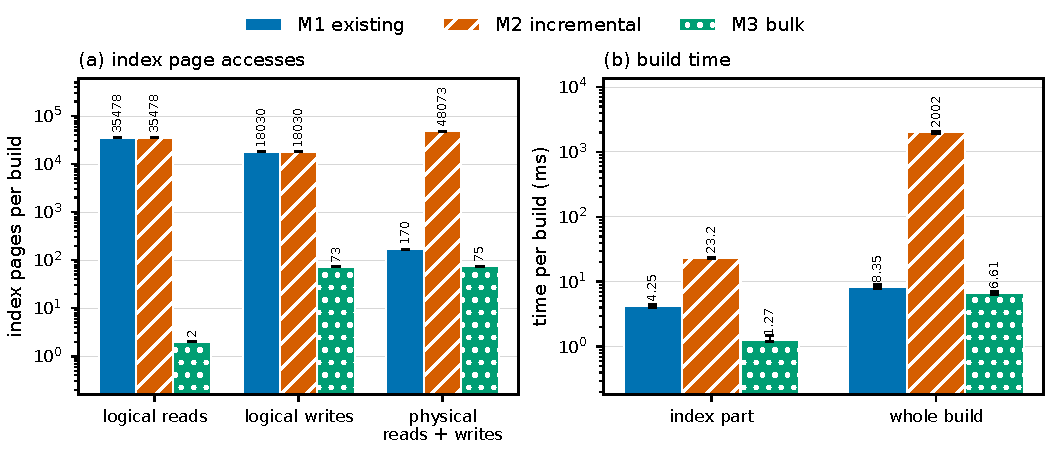
\includegraphics[width=\textwidth]{figures/index_build.pdf}
\caption{Index construction: (a) index page accesses per build, (b) build time, index part and whole build. Logarithmic axes; means over five repeats with min/max bars.}
\label{fig:indexbuild}
\end{figure}

\begin{figure}[H]
\centering
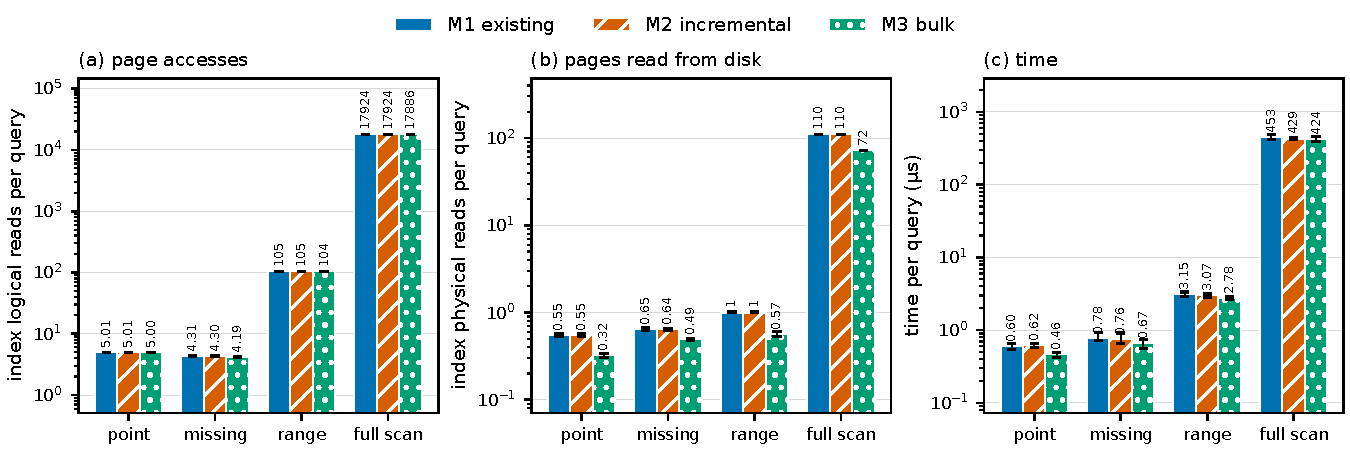
\includegraphics[width=\textwidth]{figures/index_queries.pdf}
\caption{Query cost per query type: (a) index page requests, (b) index pages read from the file, (c) time. Logarithmic axes.}
\label{fig:indexqueries}
\end{figure}

\subsection{Discussion}

\paragraph{Index size.} The bulk-loaded index has 72 pages against 110, 35\% fewer, because its leaves are 98.8\% full against 64.3\%. Insertion splits a full leaf into two halves, so an insert-built tree settles between half full and full; bulk loading fills each leaf before starting the next and never splits. Its fill is not 100\% only because the last leaf is partly empty.

\paragraph{Build cost.} Bulk loading writes each of its 72 pages once (73 writes, because page 0 is written once on creation and again as the root) and needs 2 page reads, against 35{,}478 reads and 18{,}030 writes for M1, whose every insertion descends from the root and whose splits rewrite pages. The load itself takes 1.3 ms; most of M3's 6.6 ms is the heap scan and the sort, which a pre-sorted file would not need.

\paragraph{Incremental build and buffer contention.} M2 does exactly the same index work as M1, the same logical reads and writes, yet its build takes 2 s. Almost all of it is the heap: first-fit insertion reads 4.0 million heap pages through the pool for 17{,}813 records, and those pages evict index pages from the 50 frames. The index therefore needs 31{,}905 physical reads in M2 against 30 in M1 for a tree of the same size. Measuring the two files separately is what makes this visible: the cost of incremental building here is not in the B+ tree but in the competition for the buffer pool, the same effect studied in Part 1.

\paragraph{M1 and M2 are different trees.} Both have 110 pages, 109 leaves and 64.3\% fill, but 9 of the 109 leaves hold different key ranges. M2 inserts in file order and M1 in heap-scan order, and the two differ for 31 records that first-fit placed on earlier heap pages; those keys arrive at different times, so a few leaves split at different keys.

\paragraph{Queries.} All three trees have height 2, so the number of page requests per query is almost the same. A point query costs 5 requests rather than 2 because the provided scan code also locates the leftmost leaf on every scan open, whatever the operator (2 requests, a descent since A1), and fixes the leaf again for each record id it returns (D36). The difference between the methods appears in the pages read from the file: with a cold pool, the smaller bulk-loaded tree needs 41\% fewer physical reads per point query (0.323 against 0.550), 43\% fewer per range query (0.572 against 1.000), and 72 instead of 110 for a full scan, exactly one read per index page. Times follow the same order but differ little, because the operating system's file cache serves most of these reads from memory; on a real disk the page counts would dominate (D37). Fetching the records found by the point queries costs another 0.898 heap pages per query for every method, more than the index lookup itself.

\paragraph{Fill factor.} A fill factor below 1.0 trades read cost for insert cost: at 0.5 the student index has 141 leaves and 142 pages, twice the pages to read in a range or full scan, but every leaf has room for future insertions without splitting. A fully packed bulk-loaded tree is best for a read-mostly file; the first insertion into any of its leaves forces a split.

% ---------------------------------------------------------------------
\section{Validation against analytical predictions}
\label{sec:validation}
% ---------------------------------------------------------------------

Many of the measured quantities follow from first principles, given the page size, the record and key counts and the access pattern. Table~\ref{tab:validation} compares each such prediction with the measurement. Every prediction is met exactly, up to the rounding of means over five repeats. The point-query prediction is an expectation over randomly chosen keys and is met within sampling error, as discussed below the table. Quantities that depend on the particular random sequence, such as the hot/cold hit ratios, have no simple closed form and are not listed. Agreement of this kind is a check of the implementation as well as of the analysis: an error in the replacement order, the slot arithmetic or the bulk loader's fill computation would show up as a mismatch.

\begin{table}[H]
\centering
\small
\caption{Predicted and measured values. \(p\) is the pool size in frames, \(L\) the static record length; the file of Part 1 has 1000 pages and each run 10{,}000 operations; the index holds 17{,}810 distinct keys.}
\label{tab:validation}
\begin{tabularx}{\textwidth}{Y>{\raggedright\arraybackslash}p{4.6cm}rr}
\toprule
Quantity & Prediction & Predicted & Measured \\
\midrule
\multicolumn{4}{l}{\textit{Part 1: buffer manager (all-read runs unless stated)}} \\
Uniform hit ratio, LRU, \(p = 20\) & \(p / 1000\) & 0.020 & 0.020 \\
Uniform hit ratio, LRU, \(p = 100\) & \(p / 1000\) & 0.100 & 0.100 \\
Sequential hit ratio, LRU, \(p \le 900\) & every page evicted before reuse & 0 & 0.000 \\
Sequential hit ratio, MRU, \(p = 100\) & \(9p / 10\,000\) (9 passes after the first) & 0.090 & 0.090 \\
Sequential hit ratio, MRU, \(p = 900\) & \(9p / 10\,000\) & 0.810 & 0.810 \\
Uniform and sequential hit ratio, \(p = 1200\) & \(1 - 1000 / 10\,000\) (compulsory misses only) & 0.900 & 0.900 \\
Disk I/O per operation, uniform, LRU, \(p = 100\), all writes & \(2\,(1 - 0.1)\): one read and one write-back per miss & 1.80 & 1.80 \\
Disk I/O per operation, sequential, LRU, \(p = 100\), all writes & one read and one write-back per operation & 2.00 & 2.00 \\
\midrule
\multicolumn{4}{l}{\textit{Part 2: static layout}} \\
Slots per page, \(L = 110\) & \(\lfloor 4092 / (L + 2) \rfloor\) & 36 & 36 \\
Data pages, \(L = 100\) / 110 / 256 & \(\lceil 17\,813 / \textit{slots per page} \rceil\) & 446 / 495 / 1188 & 446 / 495 / 1188 \\
Utilization, \(L = 110\) & \(1\,759\,011 / (495 \times 4096)\) & 0.868 & 0.868 \\
\midrule
\multicolumn{4}{l}{\textit{Part 3: bulk-loaded index (M3)}} \\
Leaves, fill factor 1.0 & \(\lceil 17\,810 / 254 \rceil\) & 71 & 71 \\
Index pages, fill factor 1.0 & leaves + one root & 72 & 72 \\
Leaf fill & \(17\,810 / (71 \times 254)\) & 98.8\% & 98.8\% \\
Page writes during the build & each page once, page 0 twice & 73 & 73 \\
Index pages, fill factor 0.75 / 0.5 & \(\lceil 17\,810 / \lfloor 254 f \rfloor \rceil + 1\) & 95 / 142 & 95 / 142 \\
Full scan physical reads, cold pool & one per index page (M1 / M3) & 110 / 72 & 110 / 72 \\
Point query page requests, M1 and M2 / M3 & 5, plus 1 if the key is last in a non-final leaf or has two record ids: \(5 + (\textit{leaves} - 1 + 3) / 17\,810\) & 5.006 / 5.004 & 5.006 / 5.005 \\
\bottomrule
\end{tabularx}
\end{table}

A point query normally costs 5 page requests: 2 to locate the leftmost leaf when the scan opens, 2 for the search descent and 1 to fix the leaf again for the record id. When the scan has returned the last record id of the last key in a leaf, the provided \texttt{AM\_FindNextEntry} (\texttt{amscan.c}) fixes the next leaf to load the following key before the equality test ends the scan, which costs one more request. This happens when the queried key is the last one in any leaf but the final leaf, or has a second record id. Logging every one of the 5{,}000 point queries per method confirms this: 28, 31 and 23 queries took 6 requests for M1, M2 and M3, of which 26, 29 and 21 were last keys of a non-final leaf and 2 were duplicate keys, and none took more than 6. The expected excess, \((\textit{leaves} - 1 + 3)/17\,810\), is therefore 0.006 for the 109-leaf trees and 0.004 for M3; the measured 0.0056, 0.0062 and 0.0046 differ from it only by the sampling error of 5{,}000 random queries.

% ---------------------------------------------------------------------
\section{Relation to production systems}
\label{sec:related}
% ---------------------------------------------------------------------

\paragraph{Buffer replacement.} Chou and DeWitt~\cite{chou85} showed that the best replacement policy depends on the reference pattern of each query, and that for a looping sequential reference larger than the available buffers MRU is the right choice, which is the result of Section~\ref{sec:part1}. Selecting the policy per file, as in this project, is a simple form of the same idea. Production systems address the same problem by preventing a large scan from flushing the pool rather than by switching the whole pool to MRU. PostgreSQL gives a sequential scan of a table larger than a quarter of its buffer pool a small private ring of buffers that the scan reuses, so the rest of the pool keeps its contents~\cite{pgbuf}. InnoDB inserts a newly read page 3/8 of the way from the tail of its LRU list and moves it to the head only when it is accessed again, so that pages read once by a table or index scan age out before the frequently used pages~\cite{innodb}.

\paragraph{Slotted pages.} PostgreSQL heap pages use the organization of Section~\ref{sec:part2}: a 24-byte page header, an array of 4-byte line pointers, each an (offset, length) pair, that grows from the front, and tuples that grow from the end of the page~\cite{pgpage}. A tuple is addressed by its page and line-pointer number, so tuples can be moved within the page without changing their identifiers, as in this project's record ids.

\paragraph{Bulk loading.} PostgreSQL's \texttt{CREATE INDEX} builds a B-tree bottom-up from sorted entries, and its fill factor, 90 by default for B-trees, sets the percentage to which leaf pages are filled during this initial build~\cite{pgindex}, leaving room for later inserts. This is the trade-off discussed for \texttt{bulk\_fill\_factor} in Section~\ref{sec:part3}: the value of 1.0 used here suits a read-mostly file, while a production default reserves space because later inserts are expected. Textbook treatments of slotted pages and of bulk loading B+ trees are given by Ramakrishnan and Gehrke~\cite{rg03}.

% ---------------------------------------------------------------------
\section{Changes to the provided code}
\label{sec:changes}
% ---------------------------------------------------------------------

Every change to the provided PF and AM source is marked in the code with \texttt{CHANGED [ID]}. The README contains the same table with file names and further detail.

\small
\begin{longtable}{>{\raggedright\arraybackslash}p{0.6cm}>{\raggedright\arraybackslash}p{4.3cm}>{\raggedright\arraybackslash}p{4.2cm}>{\raggedright\arraybackslash}p{5.2cm}}
\toprule
ID & Change & Reason & Consequence if not made \\
\midrule
\endhead
B1 & One top-level Makefile; provided code built with \texttt{-std=gnu89}. & The provided sources are pre-ANSI C. & The code does not compile with a current gcc (32, 47 and 19 errors in \texttt{buf.c}, \texttt{pf.c}, \texttt{hash.c}). \\
B2 & The stale \texttt{amlayer/pf.h} removed; one shared \texttt{pf.h}. & The copies disagreed on the page size (1020 against 4096 bytes). & B+ tree nodes use a quarter of each page; Part 3 page counts about four times too large. \\
P1 & Pool allocated at run time from \texttt{buffer\_pool\_size}; \texttt{PF\_InitBuffer(n)}. & The pool size must be configurable. & Each pool size needs a recompile, which the submission rules forbid. \\
P2 & Hash table enlarged from 20 to 1031 buckets. & Pools of 50 to 1200 frames. & Long hash chains add cost to every page lookup. \\
P3 & Policy per open file; \texttt{PF\_OpenFileEx(name, policy)}; MRU victim search from the head. & LRU and MRU must be selectable at open. & No way to choose the policy. \\
P4 & \texttt{PF\_OpenFile} kept as a wrapper using the default policy. & Existing callers. & Every AM caller and provided test would need editing. \\
P5 & \texttt{PF\_MarkDirty(fd, page)}, without changing recency. & An explicit mark-dirty call is required. & The dirty bit can only be set through unfix. \\
P6 & Per-file and global I/O counters; \texttt{PF\_GetStats}, \texttt{PF\_ResetStats}, \texttt{PF\_PrintStats}, \texttt{PF\_FlushAll}. & Statistics are required in all three parts. & No I/O can be measured. \\
P7 & Debug prints use \texttt{\%p} for pointers. & 64-bit pointers. & Truncated pointer values in debug output. \\
A1 & \texttt{GetLeftPageNum} descends from the root. & Page 2 is the leftmost leaf only in insert-built trees. & Scans of bulk-loaded trees skip the first leaf or fail. \\
A2 & \texttt{AM\_BulkLoad} added (\texttt{amlayer/ambulk.c}); no existing function changed. & Part 3 requires a bulk-loading method. & No bulk-loaded index to compare in Part 3. \\
A3 & The \(\ne\) scan updates its current key when skipping. & The skip was undone by a consistency check. & \(\ne\) scans return the excluded key or fail at a leaf boundary. \\
A4 & A \(\ne\) scan always initialises its cursor at the leftmost leaf. & For an absent value the cursor kept an earlier scan's state. & All 4{,}807 test probes failed: wrong record ids, garbage codes or crashes. \\
A5 & Moving past the last key of a leaf releases the page actually fixed; \(<\), \(\le\), \(\ne\) read the leftmost leaf from the search buffer. & The wrong page was released after the header was overwritten. & Missing-key queries in a gap between leaves fail and leave two pages fixed (95 of 95 probes). \\
A6 & \(<\) and \(\le\) scans stay ended once over. & The end-of-range check reset a finished scan. & \(\le\) on the largest key returns about twice the records or garbage. \\
A7 & The early stop of \(<\) and \(\le\) compares page numbers for equality, not order. & Page numbers are not in leaf order in insert-built trees. & \(<\) on the first key of a leaf returns nothing (for example 0 of 509 records). \\
\bottomrule
\end{longtable}
\normalsize

Behaviour of the provided code that was deliberately left unchanged: no merging of nodes on deletion, 50/50 leaf splits, a single global scan table, the local \texttt{bcopy} definition, an unused debug routine (\texttt{AM\_DumpLeafPages}) that reads a variable before setting it, and the side effect of a failed close described in Section~\ref{sec:part1}. None affects the results, and changing them would alter the baseline against which bulk loading is compared (D12, D28).

% ---------------------------------------------------------------------
\section{Requirement coverage}
% ---------------------------------------------------------------------

\small
\begin{longtable}{>{\raggedright\arraybackslash}p{6.6cm}>{\raggedright\arraybackslash}p{5.6cm}l}
\toprule
Requirement & Where it is met & Status \\
\midrule
\endhead
Page buffering in the PF layer & Section~\ref{sec:part1}; P1 & Done \\
LRU and MRU replacement & P3; \texttt{test\_policy}, \texttt{stress\_pool} & Done \\
Strategy selectable when opening a file & \texttt{PF\_OpenFileEx} & Done \\
Dirty flag and explicit call to mark a page updated & \texttt{PF\_MarkDirty}; P5 & Done \\
Buffer pool size configurable & \texttt{buffer\_pool\_size}; P1 & Done \\
Statistics: pages accessed, logical and physical I/O & Table~\ref{tab:counters}; P6 & Done \\
Statistics for different read/write mixtures & Seven read percentages, Section~\ref{sec:part1} & Done \\
Graph: x = read/write mixture, y = statistics & Figures~\ref{fig:iomix} and~\ref{fig:iobreak} & Done \\
Slotted pages for variable-length records & Section~\ref{sec:part2} & Done \\
Insertion, deletion, sequential scan & Heap file API; \texttt{test\_hf} & Done \\
Used to manage the student data & \texttt{test\_hf\_load}, \texttt{bench\_space} & Done \\
Space utilization compared with static management & Table~\ref{tab:space} & Done \\
Table over different maximum record lengths & Table~\ref{tab:space}, seven lengths & Done \\
Index built from an existing file in one operation & Section~\ref{sec:part3} & Done \\
Index built incrementally & Section~\ref{sec:part3} & Done \\
Bulk loading from a sorted file & Section~\ref{sec:part3}; A2 & Done \\
Comparison: query completion time, pages accessed & Table~\ref{tab:index} & Done \\
Commented code & All new code; \texttt{CHANGED [ID]} markers & Done \\
README with description, compile and run steps & \texttt{README.md}; Appendix~\ref{app:build} & Done \\
\bottomrule
\end{longtable}
\normalsize

% ---------------------------------------------------------------------
\section{Limitations and threats to validity}
\label{sec:limits}
% ---------------------------------------------------------------------

\begin{itemize}
\item \textbf{Times.} Query times are in microseconds and include the operating system's file cache, and the processor mixes performance and efficiency cores without pinning. Times are therefore reported only to show order; the conclusions rest on page counts, which are deterministic for a given configuration (D37).
\item \textbf{One data file.} The student records have a narrow range of lengths (mean 98.75 bytes, maximum 108). The gap between the slotted and the static layouts grows with the spread between the mean and the maximum length, so data with more varied records would favour the slotted layout more strongly than Table~\ref{tab:space} shows.
\item \textbf{One pool size in Part 3.} The index comparison uses a pool of 50 frames. The cost of incremental building in M2 comes from heap pages competing with index pages for the pool, so it depends on the pool size; a pool large enough for both files would remove most of it.
\item \textbf{Tree height.} At 17{,}813 records all three trees have height 2, so the number of page requests per lookup cannot separate the methods. With up to 341 children per internal node, an insert-built tree of about 163 keys per leaf reaches height 3 at roughly 56{,}000 records, a fully packed bulk-loaded tree only at roughly 87{,}000; between these sizes bulk loading would also save one page request per lookup.
\item \textbf{First-fit heap insertion.} The slotted heap file inserts first-fit and examines every data page, because a deletion can free space on any page and records differ in size. The static file can keep a hint to the first page with a free slot, which is exact when all slots have the same size. A free-space map, such as PostgreSQL keeps for every table, would reduce the 4.0 million heap page reads of M2 to a few page requests per insertion. It was not added because it does not change the space comparison of Part 2, but it would remove most of the buffer contention measured in Part 3.
\item \textbf{Synthetic buffer workloads.} The three access patterns of Part 1 isolate the behaviour of each policy; real workloads mix patterns, which is the case the per-file policy is meant for.
\item \textbf{Scope.} There is no concurrency control and no recovery: a dirty page reaches the file only on eviction, on close or through \texttt{PF\_FlushAll}, so a crash loses it. Both are outside the scope of the assignment.
\end{itemize}

% ---------------------------------------------------------------------
\section{Conclusion}
% ---------------------------------------------------------------------

The buffer manager now has a configurable pool, LRU and MRU chosen per file, an explicit dirty flag and exact I/O statistics, all verified against an independent model. The experiments confirm the expected behaviour of the two policies with exact numbers: LRU wins when a working set is reused, MRU wins on repeated sequential scans, and the read/write mixture changes only the write-back cost, not the number of pages read. The slotted page layout stores the student table without loss at 95\% space utilization, while a static layout either truncates records or wastes space in proportion to the gap between the average and the maximum record length. For the index, bulk loading from sorted input builds a tree 35\% smaller, with full leaves, at a small fraction of the build I/O of insertion, and answers every query type with fewer pages read from the file; at height 2 all three trees need the same number of page requests per lookup. Incremental construction is dominated not by the index but by the heap file competing for the buffer pool.

% ---------------------------------------------------------------------
\phantomsection\addcontentsline{toc}{section}{References}
\begin{thebibliography}{9}
\bibitem{chou85} H.-T. Chou and D. J. DeWitt. An evaluation of buffer management strategies for relational database systems. In \emph{Proceedings of the 11th International Conference on Very Large Data Bases (VLDB)}, pages 127--141, 1985.
\bibitem{pgbuf} The PostgreSQL Global Development Group. PostgreSQL source code, \texttt{src/backend/storage/buffer/README} (buffer ring replacement strategy) and \texttt{src/backend/access/heap/heapam.c}.
\bibitem{innodb} Oracle. \emph{MySQL 8.4 Reference Manual}, Section 17.8.3.3, Making the Buffer Pool Scan Resistant. \url{https://dev.mysql.com/doc/refman/8.4/en/innodb-performance-midpoint_insertion.html}
\bibitem{pgpage} The PostgreSQL Global Development Group. \emph{PostgreSQL Documentation}, Database Page Layout. \url{https://www.postgresql.org/docs/current/storage-page-layout.html}
\bibitem{pgindex} The PostgreSQL Global Development Group. \emph{PostgreSQL Documentation}, CREATE INDEX, storage parameter \texttt{fillfactor}. \url{https://www.postgresql.org/docs/current/sql-createindex.html}
\bibitem{rg03} R. Ramakrishnan and J. Gehrke. \emph{Database Management Systems}, 3rd edition. McGraw-Hill, 2003.
\end{thebibliography}

% ---------------------------------------------------------------------
\appendix
\section{Building and running}
\label{app:build}
% ---------------------------------------------------------------------

Requirements: gcc, GNU make, and for the figures Python 3 with matplotlib. The data archive \texttt{data.tar.gz} is extracted next to the repository, so that the configured path \texttt{../data/student.txt} resolves; alternatively \texttt{data\_file} in \texttt{toydb.conf} can be set to an absolute path.

\begin{lstlisting}
make                 # build the PF and AM layers
make test            # build and run every test program
make bench           # Part 1 benchmark  -> results/bench_buffer.csv
make plots           # Part 1 and Part 3 figures and tables
make bench-space     # Part 2 comparison -> results/bench_space.csv
make bench-index     # Part 3 benchmark  -> results/bench_index.csv
make stress          # randomized buffer model test, 20 seeds (slow)
make clean           # remove build outputs
\end{lstlisting}

All results used in this report are also committed in \texttt{results/}.

% ---------------------------------------------------------------------
\section{Configuration keys}
\label{app:config}
% ---------------------------------------------------------------------

\small
\begin{longtable}{>{\raggedright\arraybackslash}p{3.6cm}>{\raggedright\arraybackslash}p{3.7cm}>{\raggedright\arraybackslash}p{7.1cm}}
\toprule
Key & Value in \texttt{toydb.conf} & Meaning \\
\midrule
\endhead
\texttt{buffer\_pool\_size} & 50 & Frames in the buffer pool (minimum 8; built-in default 20). \\
\texttt{default\_policy} & LRU & Policy used by \texttt{PF\_OpenFile}: LRU or MRU. \\
\texttt{data\_file} & \texttt{../data/student.txt} & Student data file. \\
\texttt{work\_dir} & \texttt{/tmp/toydb\_run} & Directory for benchmark scratch files. \\
\texttt{seed} & 42 & Base seed of all random choices. \\
\texttt{repeats} & 5 & Repeats per configuration (Parts 1 and 3). \\
\midrule
\texttt{buf\_file\_pages} & 1000 & Pages in the Part 1 benchmark file. \\
\texttt{buf\_queries} & 10000 & Operations per run. \\
\texttt{buf\_pool\_sizes} & 20, 50, 100, 900, 1200 & Pool sizes measured. \\
\texttt{buf\_read\_pcts} & 100, 90, 75, 50, 25, 10, 0 & Read percentages measured. \\
\texttt{buf\_patterns} & uniform, hotcold, sequential & Access patterns measured. \\
\texttt{hot\_fraction}, \texttt{hot\_prob} & 0.2, 0.8 & Hot set size and share of accesses to it. \\
\texttt{plot\_pool}, \texttt{plot\_read\_pct} & 100, 50 & Pool and read percentage for Figures~\ref{fig:iomix}, \ref{fig:iobreak} and Table~\ref{tab:buffersummary}. \\
\midrule
\texttt{static\_lengths} & 100, 104, 110, 128, 160, 200, 256 & Static record lengths compared. \\
\texttt{churn\_fraction} & 0.3 & Share of records deleted and reinserted. \\
\midrule
\texttt{bulk\_fill\_factor} & 1.0 & Fill factor of the bulk loader, leaves and internal nodes, in (0, 1]. \\
\texttt{idx\_point\_queries} & 1000 & Point queries on existing keys. \\
\texttt{idx\_missing\_queries} & 100 & Point queries on absent keys. \\
\texttt{idx\_range\_queries}, \texttt{idx\_range\_len} & 200, 100 & Range queries and keys per range. \\
\bottomrule
\end{longtable}
\normalsize

% ---------------------------------------------------------------------
\section{Design decision log}
\label{app:decisions}
% ---------------------------------------------------------------------

Each decision taken in the project, with its reason and the consequence of not taking it. Changes to the provided code are listed separately in Section~\ref{sec:changes}. The same log, with commit and source-line references, is in \texttt{docs/DECISIONS.md}.

\small\renewcommand{\arraystretch}{1.05}
\begin{longtable}{>{\raggedright\arraybackslash}p{0.7cm}>{\raggedright\arraybackslash}p{5.2cm}>{\raggedright\arraybackslash}p{4.4cm}>{\raggedright\arraybackslash}p{4.3cm}}
\toprule
ID & Decision & Reason & If not taken \\
\midrule
\endhead
\multicolumn{4}{l}{\textit{Build, configuration and testing}} \\
D1 & One top-level Makefile; provided code compiled as gnu89, new code with all warnings and kept warning-free. & The provided code is K\&R C, rejected by current compilers. & Nothing compiles on a current gcc; new warnings hidden among old ones. \\
D2 & One \texttt{pf.h} shared by PF and AM. & The two copies had drifted to different page sizes. & The B+ tree built for a 1020-byte page on 4096-byte pages. \\
D3 & Every tunable is a key in \texttt{toydb.conf}, overridable on the command line. & Only the configuration file may change after submission. & Varying any experiment would need a code change. \\
D4 & \texttt{make test} passes for any valid configuration; a strict mode checks documented defaults. & An evaluator may edit the configuration and rerun the tests. & A legitimate edit makes the tests fail and looks like broken code. \\
D5 & Each test runs in a scratch directory with a timeout and passes only on its expected last line. & Provided test programs return garbage exit codes. & False passes, stray files, or a hung test run. \\
D6 & Data-dependent tests find the data relative to the repository and print a visible SKIPPED note if it is missing. & Tests run in a scratch directory. & Failures on every fresh checkout, or a silent skip. \\
D7 & Hand-computed expected values everywhere, plus randomized tests against independent models. & Comparing a program with its own output proves nothing. & Plausible but wrong results pass unnoticed. \\
\multicolumn{4}{l}{\textit{Part 1: buffer manager}} \\
D8 & The victim is chosen by the policy of the file whose page is being loaded, from any file. & One pool is shared by files with different policies. & A per-file policy would have no defined meaning. \\
D9 & A page moves to the head of the list when loaded and when unfixed; a hit does not move it. & Matches the provided list discipline and gives an exact, testable order. & LRU and MRU would have no precise definition. \\
D10 & Only writing a page back clears its dirty flag; a clean unfix never does. & An explicit mark-dirty call is required. & An earlier modification could be lost silently. \\
D11 & Reads, hits and misses are charged to the requested page's file, evictions and write-backs to the victim's file; one logical write per fix. & Each counter has one meaning; hits + misses = logical reads exactly. & Double counting or wrong attribution. \\
D12 & The side effect of a failed close in the provided code is documented, not changed. & No requirement depends on it. & An unrequired change to provided code. \\
D13 & Benchmark: three access patterns, five pool sizes, seven read mixes, five repeats. & The patterns separate the policies in both directions; uniform is the control. & One pattern shows only one side. \\
D14 & All policies, pool sizes and read mixes see the same page sequence. & Replacement ignores the dirty flag, so only the write cost may vary with the mix. & Random differences appear as effects on the graph. \\
D15 & Physical writes reported before and after a final flush. & Large pools evict nothing. & Write cost of large pools invisible. \\
D16 & Figures sized for the report, colour-blind-safe, readable in greyscale, reproducible. & Readability. & -- \\
\multicolumn{4}{l}{\textit{Part 2: slotted pages and static management}} \\
D17 & Record id = page \(\times\) 4096 + slot; records over 1024 bytes rejected. & One integer the B+ tree can store. & -- \\
D18 & Utilization = bytes of record content stored / (data pages \(\times\) 4096), the same for both layouts. & A fair comparison. & Static utilization inflated by counting slot capacity (it reversed the result in the first version). \\
D19 & A record is a line without its terminator; CRLF stripped; lines without 16 fields skipped. & The terminator is a file-format artifact. & Every record one byte too long. \\
D20 & Tests assert invariants, not numbers of one data file. & The data file may be replaced. & Any other valid file makes the tests fail. \\
D21 & Static slots store a 2-byte length (top bit = truncated) before \(L\) bytes. & Variable-length records in fixed slots need their length. & Wrong utilization; deletes cannot update statistics. \\
D22 & Static lengths 100 to 256 compared; 108 is the longest record. & Shows both truncation and waste. & -- \\
D23 & Churn: delete 30\% at random and reinsert. & Shows whether freed space is reused. & -- \\
\multicolumn{4}{l}{\textit{Part 3: B+ tree index}} \\
D24 & Index key: roll number as \texttt{char(8)}. & Roll numbers contain letters and leading zeros. & An integer key rejects or corrupts them. \\
D25 & The leftmost leaf is found by descending from the root (A1). & Needed for any tree not built by insertion. & Scans of bulk-loaded trees skip data. \\
D26 & The not-equal skip fixed (A3), found by the test for A1. & Wrong answers on any tree. & \(\ne\) scans return the excluded key. \\
D27 & Bulk loader: root in page 0, leaves in pages \(1 \ldots k\), fill factor from the leaf byte capacity, a key's record ids in one leaf. & The AM layer assumes the root is page 0; the fill factor must mean what it says. & Unreachable pages and a fill-factor experiment that measures nothing. \\
D28 & Other provided AM behaviour left unchanged (no merge on delete, 50/50 splits, one scan table). & None affects the results. & The baseline for bulk loading would change. \\
D29 & Three build methods measured on identical data. & Requirement of Part 3. & -- \\
D32 & Index and heap I/O measured separately and checked against the global totals. & Heap insertion cost would swamp the index comparison. & M2 would look slow for reasons unrelated to the index. \\
D33 & All three indexes answer one identical query set, every result checked against a sorted copy. & A fair and verified comparison. & Differences caused by different queries, or unnoticed wrong answers. \\
D34 & Every build and every query batch starts from a cold pool. & Pages cached by an earlier phase would hide real costs. & Later methods would look cheaper only because of a warm pool. \\
D35 & The four scan bugs found by the bulk-loader review fixed as A4 to A7 with failing-first tests. & Missing-key and boundary queries are part of the workload. & Wrong results and pages left fixed during measurement. \\
D36 & The provided behaviour of locating the leftmost leaf on every scan open is documented, not changed. & It costs the same for all three methods. & Another change to provided code with no effect on the comparison. \\
D37 & Page counts are the primary metric; times are reported with the caveat of the OS file cache. & Physical reads here are mostly served from memory (41\% fewer reads per point query, only 23\% less time). & Small time differences misread as small real costs. \\
\multicolumn{4}{l}{\textit{Process}} \\
D30 & Code changes on their own branch, merged by pull request after checks chosen for the change; setup, documentation and results commits go directly to the main branch. & A reviewable history and no unverified code on the main branch. & -- \\
D31 & Benchmarks validate input before producing output and keep the previous results on failure. & A partly written results file looks valid. & Half-written or silently wrong results. \\
\bottomrule
\end{longtable}
\normalsize

\end{document}
